\documentclass{article}
\usepackage[utf8]{inputenc}
%\usepackage[english, ngerman]{babel}
\usepackage{array}
\usepackage{float}
\usepackage{graphicx}
\usepackage[dvipsnames]{xcolor}
\usepackage[numbers]{natbib}
\usepackage{csquotes}
\usepackage[numbib]{tocbibind}
\usepackage{dirtytalk}
\usepackage{listings}
\usepackage{xcolor}
\usepackage{multicol}
\usepackage{multirow}
\usepackage{wrapfig}

\colorlet{punct}{red!60!black}
\definecolor{background}{HTML}{EEEEEE}
\definecolor{delim}{RGB}{20,105,176}
\colorlet{numb}{magenta!60!black}

\lstdefinelanguage{json}{
    basicstyle=\normalfont\ttfamily,
    numbers=left,
    numberstyle=\scriptsize,
    stepnumber=1,
    numbersep=8pt,
    showstringspaces=false,
    breaklines=true,
    frame=lines,
    backgroundcolor=\color{background},
    literate=
     *{0}{{{\color{numb}0}}}{1}
      {1}{{{\color{numb}1}}}{1}
      {2}{{{\color{numb}2}}}{1}
      {3}{{{\color{numb}3}}}{1}
      {4}{{{\color{numb}4}}}{1}
      {5}{{{\color{numb}5}}}{1}
      {6}{{{\color{numb}6}}}{1}
      {7}{{{\color{numb}7}}}{1}
      {8}{{{\color{numb}8}}}{1}
      {9}{{{\color{numb}9}}}{1}
      {:}{{{\color{punct}{:}}}}{1}
      {,}{{{\color{punct}{,}}}}{1}
      {\{}{{{\color{delim}{\{}}}}{1}
      {\}}{{{\color{delim}{\}}}}}{1}
      {[}{{{\color{delim}{[}}}}{1}
      {]}{{{\color{delim}{]}}}}{1},
}
\def\arraystretch{1.5}%  1 is the default, change whatever you need

\newcolumntype{P}[1]{>{\raggedright\arraybackslash}p{#1}}
\newcolumntype{M}[1]{>{\centering\arraybackslash}m{#1}}

%\renewcommand{\bibsection}{\section*{Literaturverzeichnis}}




\title{}
\author{Santiago Moreno}
\date{August 2022}
\begin{document}
\begin{titlepage}
\begin{center}

\begin{figure}
\centering

\includegraphics[width=0.25\textwidth]{img/ZHAW_Logo.png} %
\end{figure}

\vspace*{.06\textheight}
\vspace{1.5cm} 
\textsc{\Large Master Thesis}\\[0.5cm] % Thesis type

\hrule% Horizontal line
\vspace{0.4cm}
\huge Remote Collaboration in Augmented Reality \vspace{0.4cm} % Thesis title
\hrule % Horizontal line
\vspace{0.4cm}

\begin{minipage}[t]{0.4\textwidth}
\begin{flushleft} \large
\emph{Author:}\\
Santiago Moreno% Author name - remove the \href bracket to remove the link
\end{flushleft}
\end{minipage}
\begin{minipage}[t]{0.4\textwidth}
\begin{flushright} \large
\emph{Supervisor:} \\
Philipp Ackermann % Supervisor name - remove the \href bracket to remove the link  
\end{flushright}
\end{minipage}\\[3cm]
 
\vfill

\large \textit{}\\[0.3cm] % University requirement text
\textit{}\\[2.4cm]

\vfill

{\large \today}\\[4cm] % Date
%\includegraphics{Logo} % University/department logo - uncomment to place it
 
\vfill
\end{center}
\end{titlepage}
\begin{center}
    \Large
    \textbf{Abstract}
    
\end{center}

The goal of this thesis was to establish and explore a general-purpose AR-to-Video collaboration functionality in the context of indoor spaces. For this, the existing AR application ARchi VR was used as a basis. The implemented features enable remote users to interact with the onsite user's environment as if they were physically present. Additionally, the potential of these established collaboration functionalities are explored through three specific use-cases: remote maintenance, remote expert assistance, and interior design.
\newpage
\begin{center}
    \Large
    \textbf{Acknowledgments}
\end{center}
I would like to extend my deepest thanks to my advisor Dr. Philipp Ackermann for the helpful advice, in-depth code reviews and new features for ARchi VR he provided during the whole project.
\newpage
\tableofcontents
\newpage

\section{Introduction}
The demand for remote work capabilities is steadily rising among many employees. The contemporary standard for communication when collaborating with an on-site colleague is to use VoIP software such as Teams or Zoom. There is great potential in increasing efficiency and quality of such a session by improving the collaboration tools used.\\
Using AR (Augmented Reality) in a spatial context greatly improves a user's understanding of the surrounding scene, which also applies to remote participants.
By allowing remote users to directly annotate into the on-site physical space through a received video stream, gives them an intuitive way of conveying information and ideas. There already exist numerous successful commercial collaboration solutions, that utilize such an AR-to-Video approach during collaboration, such as Microsoft Dynamics 365 Remote Assist or TeamViewer's xAssist.\\
The goal of this thesis is to establish and explore a general-purpose AR-to-Video collaboration functionality in the context of indoor spaces. For this, the existing AR application ARchi VR will be used as a basis. \\
The following subchapters introduce the reader to all necessary technical concepts. The passages incorporate text from previously written works as well as a paper, that was published and presented at the MUC Conference in Rapperswil during the course of this thesis. These sections have been revised and restructured to give the reader a comprehensive overview. 

\subsection{ARchi VR}
ARchi VR is a room-scanning app for iOS developed by Philipp Ackermann. Originally developed with mainly the use-case of architecture in mind, it has since been expanded to encompass a broader set of features, with a main focus on indoor spaces.\\
\subsubsection{Capturing a Room}
Interaction with a room in ARchi VR begins with the definition of its boundaries. To do so, the user first determines the floor as a plane by pointing the camera of their phone towards the ground. The app detects the floor through feature detection. The next step is to define the room's walls, which can be accomplished in two ways. The first is to manually set the desired walls by pointing the camera towards each corner, consecutively marking them in a circular manner. During wall creation, if desired, an optional ceiling can also be defined by pointing the camera upwards to measure its height. Once walls have been established, the last step in the manual room capture process is to define cutouts, which are openings into the room such as doors or windows. This is accomplished by selecting the two diagonal corners of a desired opening.
The second method automatically detects floor, walls, doors, windows, and furnitures by using Apple's RoomPlan API\cite{inc_roomplan_2023} in combination with a self-developed heuristic.
After capturing the room, properties can be modified for all defined cutouts or boundaries through long-tapping gestures (e.g., changing a wall's texture or changing a door's opening direction).

\subsubsection{Augmenting Rooms with Items}
After a room's basic outline has been established, users are able to place and map various augmentations to physical points in the room. Augmentations are defined and managed as Item objects. Each item is identified by its type and subtype. In general an items type defines how many points are necessary for creation, while the subtype is used for definition of its visual features. The following is a summary of the most important items.
\begin{description}
   \item[Spot Marker] Spot markers are used to draw attention to specific locations and can be placed both on walls and floors.
   \item[Panels] Panels can be utilized to add hypertext information to a room. The content of a panel can consist of text, image or video and, similar to a spot marker, is placed by selecting the desired point on either a wall or floor plane.
   \item[Route Item] Route item augmentations are defined by marking two or more consecutively connected points on a wall or floor. There are various representation options available through its subtypes, such as the arrow which contains a customizable text label or the measurement line that displays the distance between the two defined points. 
   \item[Zone] Zones can be created by selecting 3 or more edge points on a floor plane to create any desired polygonal shape. This feature can be used to mark and label specific areas in the room (such as a "keep free" zone seen in Fig. 2a).
   \item[Interiors and Equipments] Boundaries of existing objects in the room can be captured as their bounding box. Similar to zones, object footprints are defined through a polygonal shape, but with the addition of a height property.\\
   ARchi VR also provides various 3D models through an item catalog. The virtual 3D models can be placed anywhere in the room. Users have the ability to add their own 3D model catalog as a custom extension.
\end{description}
All of the above defined augmentations can be manipulated in AR by touch gestures (e.g., move, rotate) or by long-tap gestures (e.g., delete, change properties, lock). \\
Additionally, all items can be further enhanced with interactive content, such as self-captured text, image, or voice memos as well as external media referenced by URLs. Enhanced items are distinguished from normal ones through a pulsating glow. Tapping on an enhanced item opens its interactive content in a popup window.
\begin{figure}[H]
  \centering
  \includegraphics[width=\linewidth]{img/augment.png}
  \caption{A user has augmented an entryway with many of the available item types (a). The info spot marker (a, top) has been enhanced with additional information in the form of an image, which is displayed as a pop-up when tapped (b).}
  \label{screenshot:screenshare}
\end{figure}
\subsubsection{Viewing Rooms in 2D, 3D, and AR}
The app provides several alternate representations for captured rooms, such as a 2D floor plan view and a 3D view. Captured rooms can be reopened on-site in their AR representation by re-registering the stored feature point cloud.

\subsection{WebRTC}
WebRTC is an open source API developed by Google, which enables both web browsers and mobile devices to communicate in real time. 
\subsubsection{Signaling-Server}
For two devices to start communicating through WebRTC, a connection first has to be found and agreed upon by both peers. This agreement is done with two message types: Session Descriptions (SDP) and Interactive Connectivity Establishment (ICE) Candidates. The SDP contains information on the endpoints' video codec, source address and media timings. The ICE Candidate describes one possible way of connecting to a peer.\\
Signaling starts with one peer initiating an offer in the form of an SDP. The other peer then reacts to that offer by sending their answer in the same form. As soon as the initiator transmits their offer, all ICE Candidates are sequentially sent to the other peer in no particular order. Likewise on the other end, once the offer is sent, ICE candidates are sent to the initiator. Both peers keep track of the remote and local ICE candidates and SDP. Once they can agree upon one ICE Candidate both are able to utilize, a connection is established.\\
Since the peers don't have a connection yet, SDP and ICE Candidates have to be relayed by some service. Usually this is done by a server, but any communication method can be used as long a both peers receive the necessary ICE Candidates and SDP when requested \cite{mozilla_signaling_nodate}.
\subsubsection{STUN Server}
STUN (Session Traversal Utilities for NAT) is a protocol used to discover a peer's public IP address while also checking its accessibility. STUN is necessary for WebRTC once peers don't share a local network.
\subsubsection{TURN Server}
TURN servers are required when a peer is behind a router that applies symmetric NAT. This restriction prohibits connections from any endpoint that has not been previously connected to.\\
To bypass this, all communication is relayed through a TURN server, effectively making WebRTC not peer-to-peer anymore. While TURN servers are not required for WebRTC, they are highly recommended if peers need to connect from environments with stricter security rules.

\subsection{SharePlay}
SharePlay is an API and Service offered by Apple for all their newer devices (iOS/iPadOS 15+). The usage of SharePlay enables remote communication for any iOS and iPadOS app. To join a SharePlay session, all participants need to join a FaceTime call or invite each other through the Messages app.\\
To utilize SharePlay in an iOS app, developers have to implement the group activities framework. Apple provides a default group activity realization, that enables synchronized viewing of media. If other functionality is needed, custom group activities have to be developed. Server infrastructure for the communication is provided by Apple, as long as the transmitted data size and frequency does not exceed their maximum threshold (e.g., continuously sending video frames).

\subsection{Previous Results}
In the previous works “Technology Assessment for AR Collaboration” \cite{moreno_technologieabklarung_2022} and "Evaluating SharePlay and WebRTC for Real-Time Collaboration in ARchi VR"\cite{moreno_evaluating_2022}, we evaluated and implemented the basis to support synchronous collaboration for two participants in ARchi VR. The following subchapters summarize the developed architecture and functionality.

\subsubsection{Joining a session} \label{basis}
To start collaborating, users must first join a shared FaceTime call, this can be either done manually or by invitation directly in ARchi VR. Tapping on the group session icon, which is visible in any view inside a room, will create a session. The session's initiator is designated as the host of the collaboration. All other participants in the call will receive a notification once the session has been created. Joining a room can be done by tapping on the notification or through a button FaceTime offers. \\  
The session gets automatically terminated if the host decides to close the view. Furthermore, the session can be closed either through FaceTime or the group session icon. The session persists, if a non-host leaves the session.
\begin{figure}[H]
  \centering
  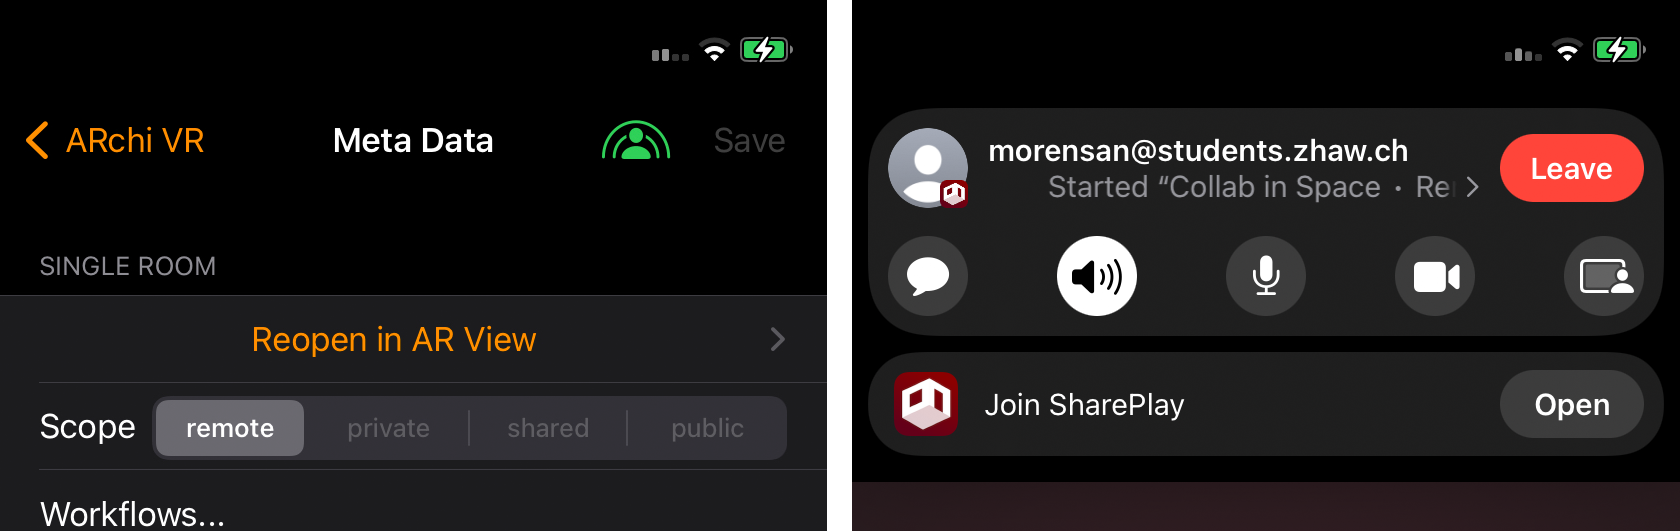
\includegraphics[width=0.7\textwidth]{img/session_join_screenshot.png}
  \caption{Cropped Screenshots illustrating the joining process. The on-site user (left) selected a room and tapped on the green group session icon to start the collaboration. The remote participant (right) in the FaceTime call receives a notification and can join the collaboration by tapping on the button labeled "Open". }\label{screenshot:join}
\end{figure}
\subsubsection{Multi-modal collaboration} \label{basis}
Users can verbally and visually communicate their intentions through the available audio and face cam streams provided by FaceTime. Furthermore, participants are able to edit the room through any of the available views. By long tapping on an item and selecting the appropriate action in the appearing popup menu, the user is able to modify its properties such as position, rotation, or color. All existing views (i.e., 2D, 3D and AR) are synchronized through SharePlay, enabling users to freely switch between them as they desire and use any of the features available (see Fig.\ref{fig:teaser}, b, c and d). A user's position and viewing direction in AR or in 3D is shared in real-time (see Fig.\ref{fig:teaser} b and c) and remotely presented as awareness clues in 2D, 3D and AR. \\
Remote participants are also able to request a video of the local user's screen in order to directly spectate the host perspective (see Fig.\ref{fig:teaser}, d). 

\subsubsection{Communication Architecture}
SharePlay is used for establishment of the session, thus removing the need to develop our own session invitation and user connection service. A custom group activity is defined and used to send data such as updates to the room.\\
Due to the data size restrictions on behalf of SharePlay, the real-time peer-to-peer communication library WebRTC is used for large volume and high frequency data such as video streams or the user's real-time position.\\ 
By using WebRTC in combination with SharePlay we avoid the need to deploy our own server hardware, which is normally required when using WebRTC. The signaling procedure is done through SharePlay, thereby eliminating the requirement for a signaling server. For STUN and TURN the free servers of OpenRelay Project were used QUOTE.


\section{Results}

\subsection{Overview}

\begin{figure}[H]
  \centering
  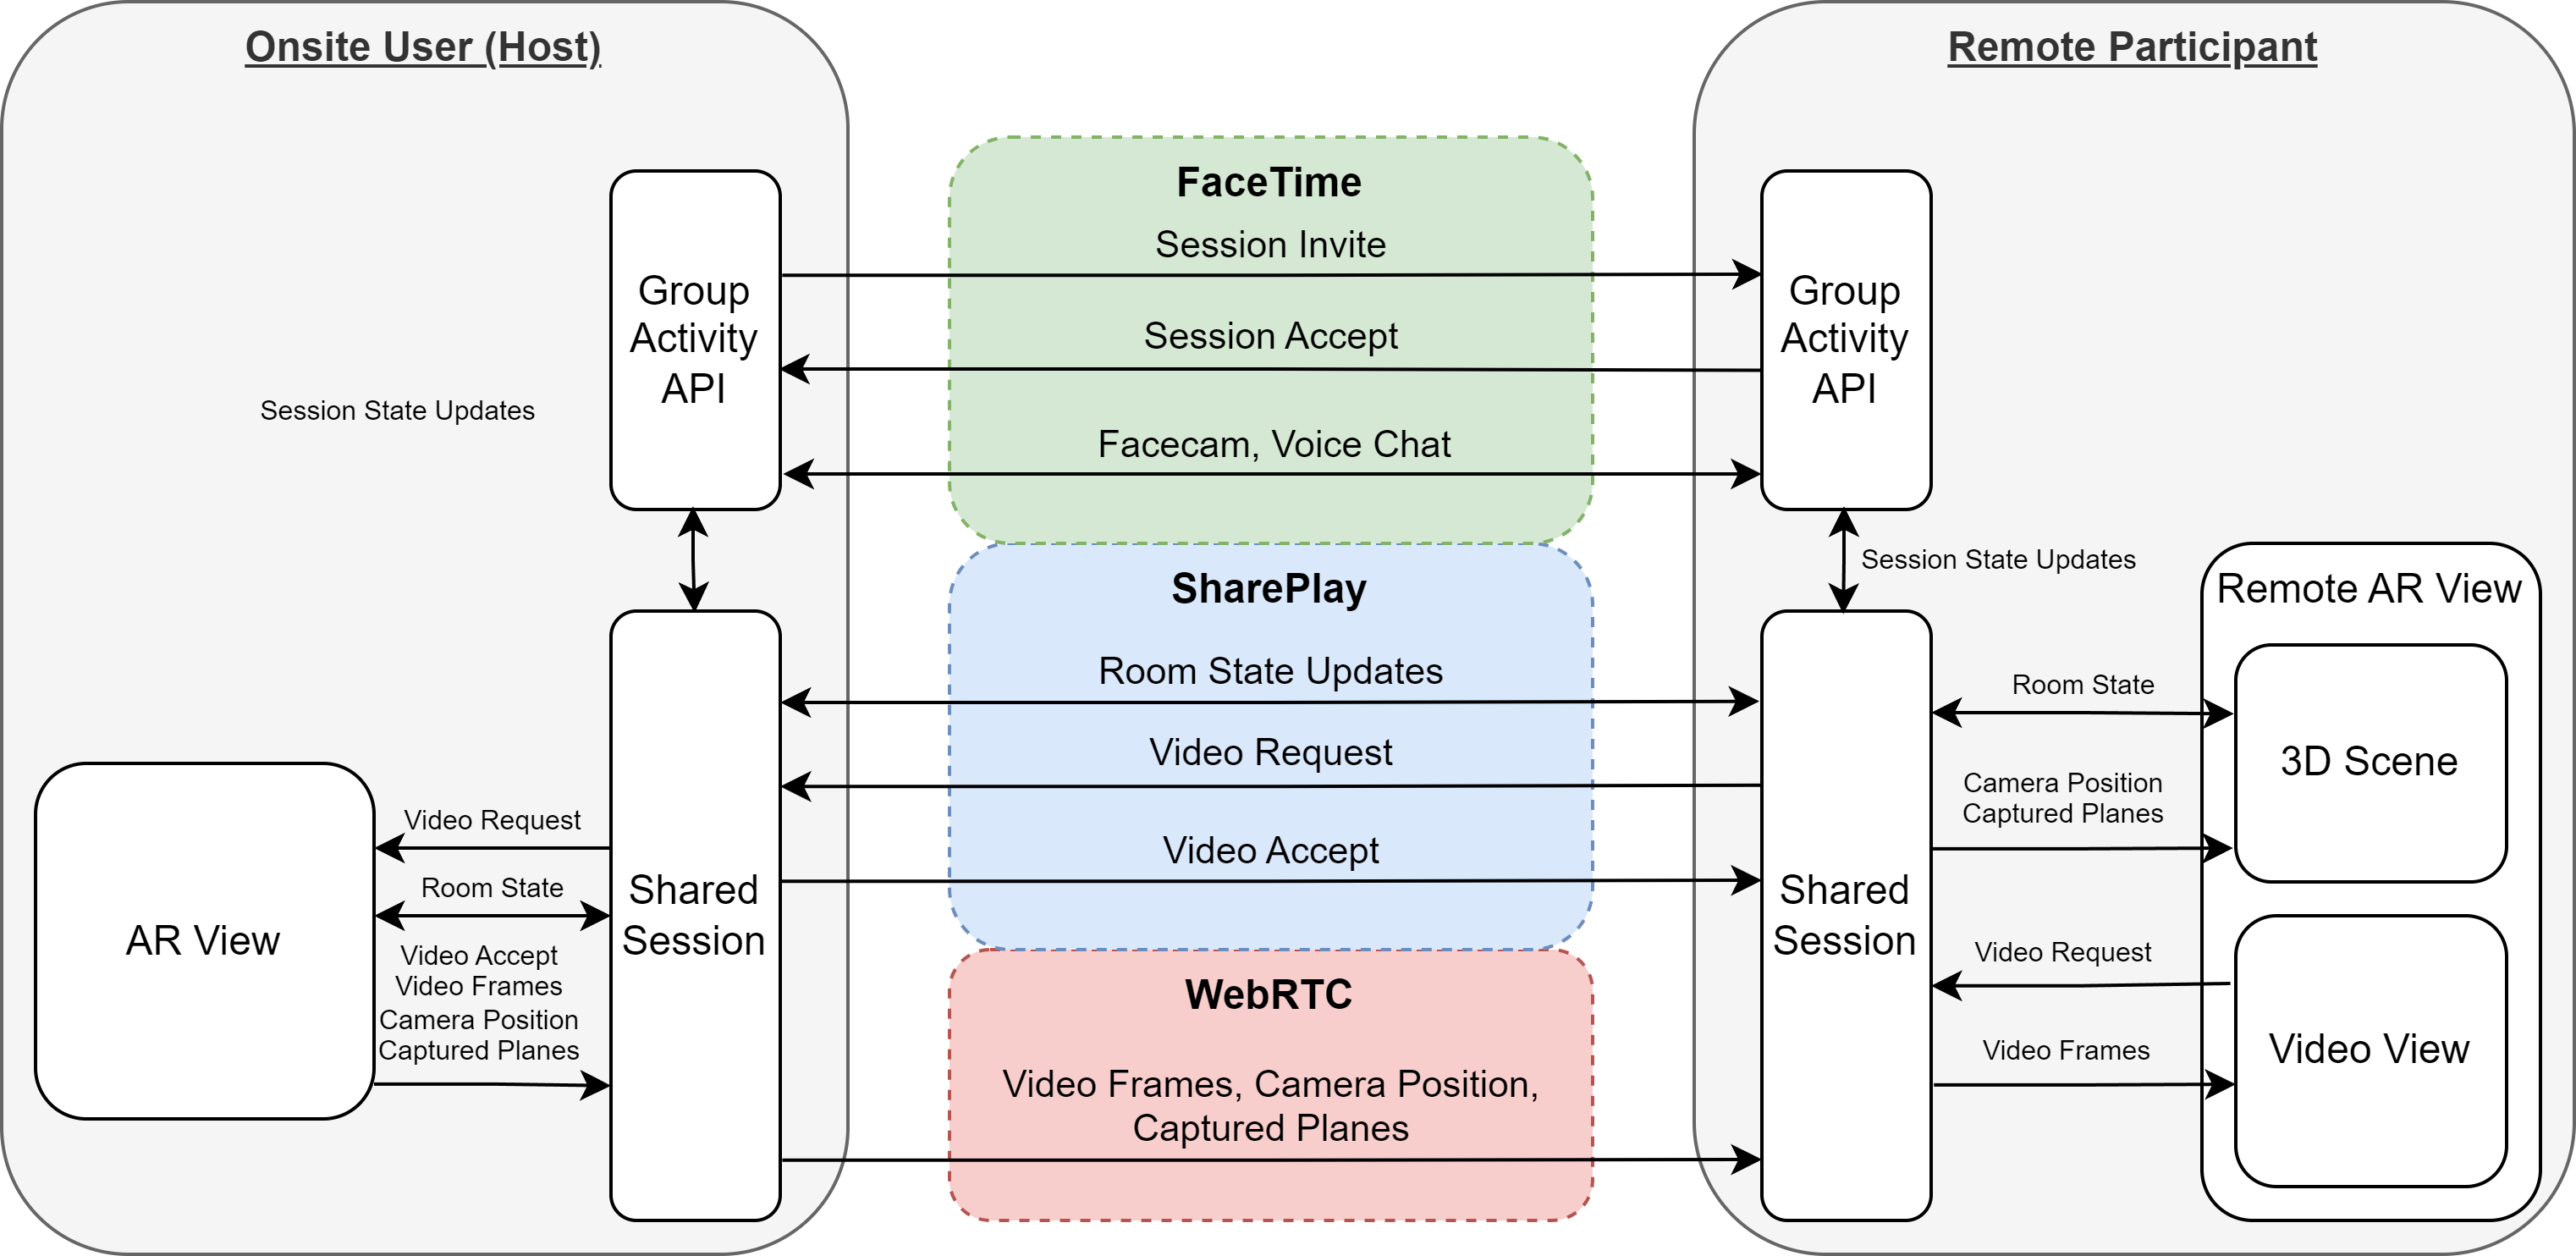
\includegraphics[width=1\textwidth]{img/architecture_system_diagram_overview.png}
  \caption{Architecture system diagram showing the data flow when two participants are collaborating the ar-to-video functionality.}
  \label{screenshot:screenshare}
\end{figure}
The implemented functionality allows a remote participant to interact with a room through a received video stream of the host's running AR session. \\
Such a session is started by the remote participant joining the host's room and requesting a video stream. The host broadcasts a non-interactive screen share to the remote participant when there is no active AR session. Once the host side opens a room in AR, the screen share is replaced with a video stream of the front facing camera (i.e., the camera used by AR). While the video stream is active, the host will also send its current camera position with each sent video frame. \\
The remote peer is notified of the switch to AR, which triggers the creation of a 3D environment that reconstructs the host's AR Scene. This includes all items, walls, cutouts and captured planes. Additionally, the received camera positions of the host are used to update the 3D environment's camera to match the current frame displayed in the video. The received video stream is overlaid by the created 3D environment, thereby effectively creating a remote AR view.\\
Any updates to the room by the host in AR are propagated to the remote participant, where they are incorporated into the 3D reconstruction. Conversely, if the remote peer makes any modifications to the room, the host is notified and updates its AR View accordingly.

\subsection{Video Frame Synchronization}
To avoid a mismatch between camera and video frame displayed, the remote peer needs to be able to synchronize them. Therefore, before being sent by the host, a unique identifier ranging from 0 to 255 is assigned to each camera position. The matching video frame incorporates this identifier as a chroma value in a rectangular area of pixels in the top right corner. The chroma value is used, as tests during development with a frame's luma value seemed to indicate more loss of information during the encoding process.\\
On each received frame, the remote peer calculates the median chroma value of the top right corner and compares the resulting identifier with all received camera positions. If there's a match, the remote AR scene is notified with the new camera position and video frame.   \\
This approach has been chosen as there currently does not exist any direct support for supplying a video frame with additional metadata in WebRTC's Library for iOS. The feature is already present on browser clients QUOTE but has never been exposed to the library of native devices and would thus require us to create and maintain a fork of the WebRTC iOS library, similarly to an example by Cao QUOTE.\\
WebRTC does supply each frame with a timestamp, unfortunately it is only accessible when receiving the frame not when sending. Additionally the timestamp is in the NTP Format, which results in it being dependent on the host devices tick-rate and potentially non-monotonic, making it hard to predict and match to real-world timestamps on the remote peer side. QUOTE?
\subsection{Handling Anchor Updates}
 AR Anchors are constantly updated to ensure that the virtual content remains accurately aligned with the real world. Therefore, changes to the hosts AR anchors have to be propagated to the remote peer to avoid misalignment of the remote AR reconstruction. \\
Taking into account the volume of anchor changes and the fact that anchors are normally updated in sporadic bursts (e.g. AR user points camera to new location) it is not feasible to inform the remote peer on each change.\\
Thus, a procedure was created to transmit anchor updates for items and captured planes in batches. An anchor update event containing all changed anchors is sent to the remote peer each $M$ milliseconds. To take the bursts into account, the procedure furthermore counts all anchor updates that occur and sends an update prematurely if the threshold $T$ has been surpassed. Constants $T$ and $M$ have been determined heuristically. After sending an update both counters are reset.\\
Two separate batch update procedures following the above explained riles have been implemented, one for updates on item anchors and the other for captured planes.
\subsection{Pausing the Video}
The remote peer has no control over the host's camera movement. This leads to both peers having to verbally coordinate all camera movements, with the host being required to hold camera positions until the remote peer has finished their interactions. To address this, a feature allowing remote participants to pause the incoming video stream was introduced. This enhancement aims to enhance autonomy and usability while minimizing the necessity for continuous coordination.\\
A pause can either be triggered manually by pressing the pause button or automatically when starting an interaction that requires minimal camera movements (i.e., editing items, drawing). When paused, both the video stream and the AR reconstructions camera are frozen. Updates to the room are still rendered. Furthermore, during pause the host's current position and viewing direction, visualized as a 3D avatar, are presented to the remote participant.
IMAGE
\subsection{Remote User Interactions}
Several interaction methods have been developed, in order to allow for direct manipulation of the room within the video view. The subsequent subchapters detail the implemented functionality.\\

\subsubsection{Item Type “Cursor”}
Many of the remote video interactions create temporary items, such as highlighting cursors or item previews. To ensure visual consistency even after anchor updates, these objects have to be defined as items in the room and propagated to the host, where it is incorporated and managed in the AR View. For this purpose, a new item type named “Cursor” was created that encompasses all the temporary items used on the remote host side. As “Cursor” items are not meant to persist, they are removed automatically from the room on host side when the AR view is closed. 

\subsubsection{Editing Items}
Editing of an existing item is triggered by tapping on the desired object. A ray cast is made from the selected location on the screen into the 3d environment to determine the selected item. The same ray cast also determines the hit captured plane behind the item, which marks it as the principal plane for this edit session. Furthermore, a grid is placed with the same orientation as the principal plane to act as a visual aid for the user.\\
After this initial setup, the video stream pauses and the editing view is displayed, wherein an item's spatial properties (i.e., rotation, position) can be manipulated through gestures. An item's rotation on the y-axis can be changed, by dragging two fingers in a rotational gesture. Through  one finger dragging gestures, the item can be moved on the principal planes surface. A straight two-finger dragging gesture allows the item to be moved perpendicular to the principal plane's surface. By anchoring item movement on the orientation of the principal plane, we allow for easier manipulation of items on walls, since single-finger dragging now corresponds to dragging it around the wall plane.\\
Additionally, an item's visual properties such as its color and text can be edited through a side-menu consisting of buttons, that trigger the corresponding popup menus. The available properties differ depending on the selected item's type, this is also reflected in the visualized buttons by hiding and showing them depending on the selected type.\\
Closing the edit view results in the video stream being resumed.

\subsubsection{Highlighting}
Remote Users can highlight a location in the room by tapping anywhere on the video with a captured plane. A ray cast is made to determine the hit plane followed by the placement of a 3D Highlighting Cursor perpendicular to the plane. The cursor's location can be changed by tapping anywhere else or by dragging it around. All changes to the cursor are immediately propagated and visualized on the host's AR View.\\

\subsubsection{Sketching}
Remote participant are able to draw directly in the room through the video view. This feature is started by tapping on the sketch button, which automatically pauses the video stream and opens the drawing menu. Drawings can then be added by the dragging gesture. As the finger moves, its position is ray cast to the corresponding location on the matching plane within the 3D environment, and a line is rendered accordingly. 
A sub-menu was defined to allow for setting of the sketches thickness and color. Furthermore, users have the option to toggle whether the drawings should persist even after the collaboration session closes.

\subsubsection{Creating Items}
In order to add new items to the room, users first have to select a location on screen. This is done through the placement of the 3D Highlighting Cursor. Once placed, a side-menu consisting of buttons for each item type is shown to the user. A temporary preview of the item is then placed at the location of the cursor by pressing on the button corresponding to the desired item type and selecting its subtype in the subsequent pop-up menu. 
The view is simultaneously switched to the edit view (s CHAPTER), which allows for further refinement of the item's position and visual properties. Users are then able to make the preview a permanent item by confirming the creation or cancelling it by closing the view, thus removing the preview either way.

\subsubsection{Drawing Zones}
The creation process of zones differs from all other items available in ARchi VR as they require the user to specify more than one location in form of  its edges. For this purpose a custom zone drawing view was created, that can be opened as soon as a plane was selected with the 3D Highlighting Cursor. Creating a new zone involves tapping to add each edge, with subsequent taps forming connecting lines to the previous ones. Alternatively a user can drag with a single finger to draw more complex shapes. Upon completing the shape, users can confirm its creation, leading to a switch to the edit view where zone properties can be further refined before finalizing its creation.


\section{Discussion}
\subsection{Exploring Results through Use-Cases}
\subsection{Video Metadata Benchmark}
\subsection{Outlook}
\newpage
\subsubsection{Usage of Mesh Data}
In its current state the Remote AR View only receives and handles the host's captured planes. While this is sufficient to allow drawing on walls and floors, planes are less useful when working with uneven surfaces, which one might find in remote maintenance situations. All newer iPhone and iPad Pro variants (iPhone Pro 12 and onwards, iPad Pro fourth generation and onwards) have LiDAR sensors installed, which enable ARKit to create a polygonal mesh of the captured physical space. ARKit partitions the captured mesh into Anchors which can be retrieved. Using these meshes on remote would allow for more realistic interaction with complex surfaces.\\

\begin{figure}[H]
  \centering
  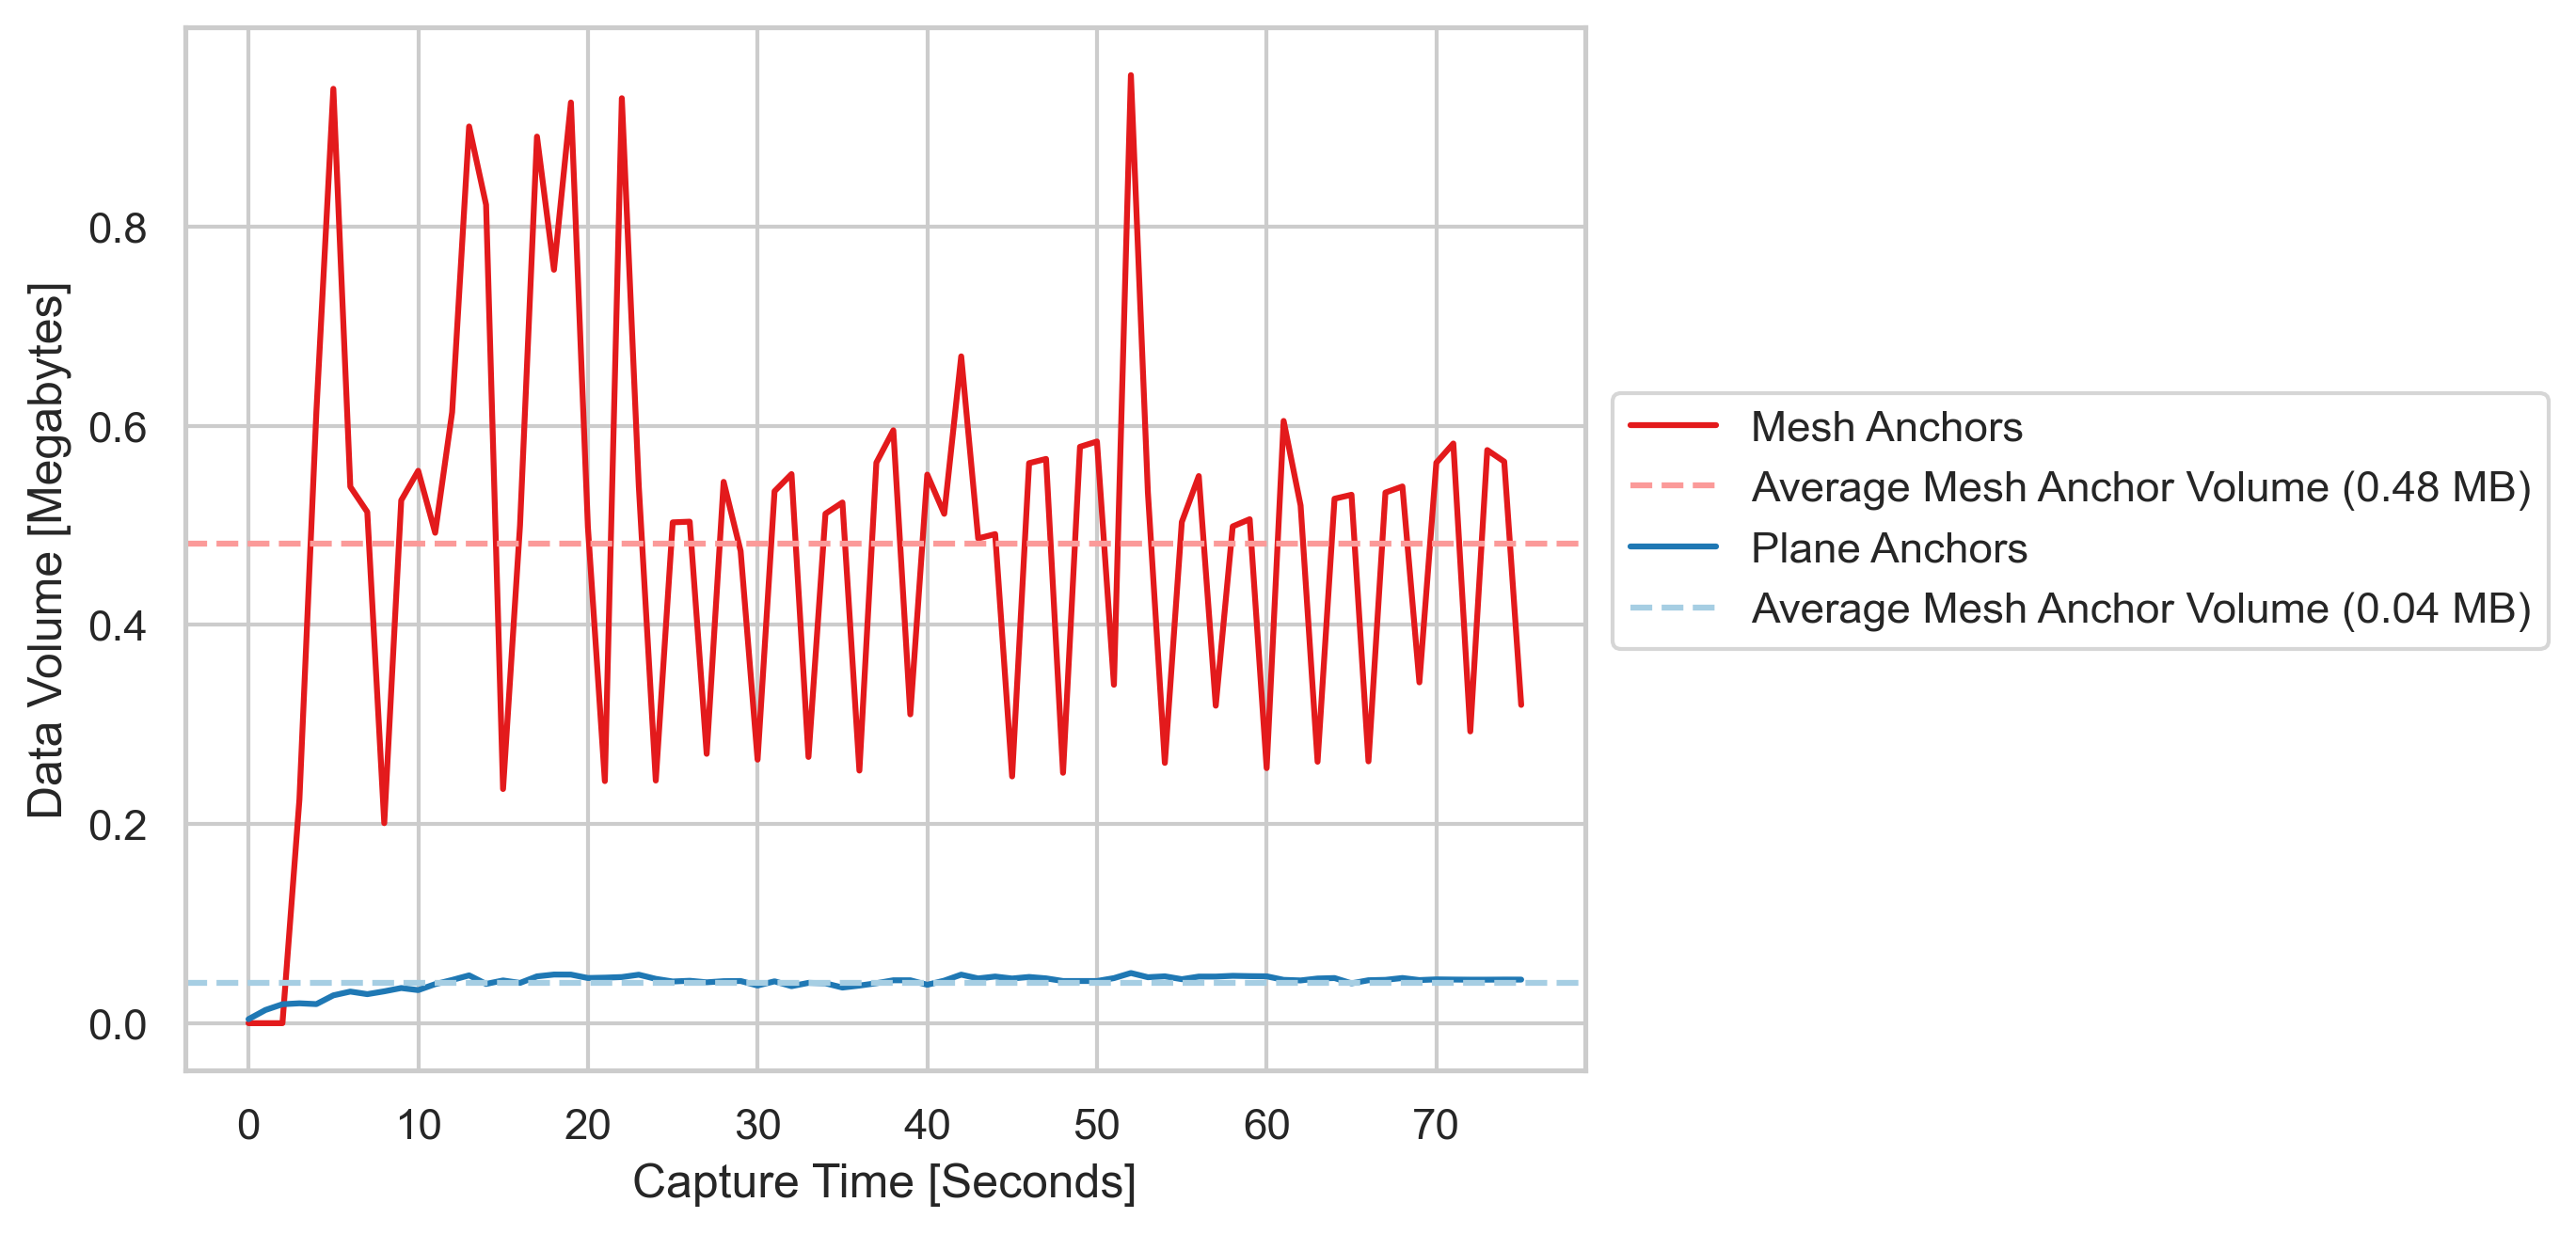
\includegraphics[width=1\textwidth]{img/mesh_plane_comparison.png}
  \caption{Measurements taken at the start of an AR Session in ARchi VR. The volume of each triggered plane and mesh anchor update has been accumulated per second.}
  \label{fig:mesh_compare}
\end{figure}

However, as shown in Figure \ref{fig:mesh_compare}, the volume of data generated with each mesh update increases by a factor of 12 when using mesh compared to plane anchors. This has to be taken into account when updating the remote peer and and the current batch transmission procedure might require more sophisticated change detection. \\
Instead of the current solution (see CHAPTER), that simply counts the number of changes to the relevant anchors since last updating the remote peer, one could keep track of all mesh anchors and count the amount of vertices that have been changed. This approach would allow for better fine-tuning of when to send an update. And would guarantee that only larger changes to the mesh would be sent in frequent intervals.

\subsubsection{"On-The-Fly" Collaboration}
ARchi VR in its current state only supports opening a shared session once a room has been defined  and saved once. For use-cases where persistent information storage is not necessary, like it is the case with remote maintenance, it would improve the user experience significantly to allow for sessions during room creation.\\
How to start such a session has yet to be determined, as a new button in the AR view would not be welcomed with the limited screen space available.
\subsubsection{Improving Planes Updating}

\subsubsection{Frame encoding efficiency}
\subsubsection{PC Client}
\subsubsection{HMD Client}
\subsubsection{Local AR-to-AR}


\subsection{Conclusion}


\newpage
\bibliographystyle{IEEEtranN}
\bibliography{references}
\end{document}
